\documentclass[11pt]{article}
\usepackage{lipsum}
\usepackage{charsheet}

\usepackage{pgfkeys}

\makeatletter
\newcommand{\runwidth}[2]{%
  % Store the macro name
  \def\@runwidth@macro{#1}%
  % Set up a key handler for "width"
  \pgfkeys{
    /runwidth/.cd,
    width/.code={
      \expandafter\@runwidth@macro\expandafter{##1}%
    },
    .unknown/.code={} % ignore everything else
  }%
  % Now parse the key-value list
  \pgfkeys{/runwidth/.cd, #2}%
}
\makeatother

\newcommand\pplabel{{\tiny PASSIVE PERCEPTION}}


\newcommand\mynode[6][white]{% fill name style+location[+fill] at contents label
  \node (#2) [#3] #4 { \Large \sffamily \mdseries #5 } ;
  \dnddecorate[#1]{#2};
  \node [outer sep=0pt, inner sep=0pt, above=of #2.south]
        {\textsf{\footnotesize #6}}
}

\newdimen\mytemp

\newcommand\newsectionenv[5][\dndrightwidth]{%
   % [width]{name}{label}{pre-code}{post-code}
  \expandafter\environbodyname\expandafter{\csname#2body\endcsname}
  \expandafter\newdimen\csname#2width\endcsname
  \NewEnviron{#2}[1][]{
    % [...] name 
    \expandafter\setlength\csname#2width\endcsname{#1-3mm}
    \node [#2,##1] (#2) {{\begin{minipage}[t]{\csname#2width\endcsname}#4\csname#2body\endcsname#5\par\medskip\hbox to \hsize{\hss\scriptsize\textsf{\strut#3}\hss}%
\end{minipage}}};
%    \dnddecorate{#2};
  }
}

\newcommand\typewidth[1]{\typeout{width is #1}}

\newcommand\newsectionenvx[5][\dndrightwidth]{%
   % [annotations]{name}{label}{pre-code}{post-code}
  \expandafter\environbodyname\expandafter{\csname#2body\endcsname}
  \expandafter\newdimen\csname#2width\endcsname
  \NewEnviron{#2}[1][]{
    % [...] name 
    %    \expandafter\setlength\csname#2width\endcsname{#1-3mm}
    \expandafter\setlength\csname#2width\endcsname{40mm}%
%    \runwidth{\typewidth}{#1}%
    \node [#2,#1,##1] (#2) {{\begin{minipage}[t]{\csname#2width\endcsname}#4\csname#2body\endcsname#5\par\medskip\hbox to \hsize{\hss\scriptsize\textsf{\strut#3}\hss}%
\end{minipage}}};
%    \dnddecorate{#2};
  }
}


\newsectionenv{magic}{MAGIC}{}{}
\newsectionenv{attacks}{ATTACKS}{}{}
\newsectionenv{features}{CLASS FEATURES}{}{}
\newsectionenvx[width=64mm,decorated clipped rectangle]{equipment}{EQUIPMENT}
   {\medskip
    \small
    \begin{minipage}{60mm}
     \begin{eqlist}}
   {\end{eqlist}
    \end{minipage}}

\tikzset{equipmentx/.style={equipment}}

\newsectionenvx[width=80mm]{equipmentx}{EQUIPMENTX}
   {\medskip
    \small
    \begin{minipage}{75mm}
     \begin{eqlist}}
   {\end{eqlist}
    \end{minipage}}

\newsectionenv[37mm]{proficiencies}{PROFICIENCIES}
   {\medskip
    \begin{minipage}{30mm}
     \begin{proflist}}
   {\end{proflist}
    \end{minipage}}

\newcommand\dndlabel[2]{% {node}{label text}
  \node [outer sep=0pt, inner sep=0pt, above=of #1.south]
        {\textsf{\footnotesize #2}};
}
\newcommand\dndtoplabel[2]{% {node}{label text}
  \node [outer sep=0pt, inner sep=0pt, below=of #1.north]
        {\textsf{\footnotesize #2}};
}
  

\begin{document}
\pagestyle{empty}

\runwidth{\typewidth}{height=frogs,draw,width=17mm,nodraw}

\newcommand\tinystacklabel[2]{\raisebox{3mm}{\tiny\begin{tabular}{c}#1\\#2\end{tabular}}}


\newcounter{proficiency bonus}
\newcounter{ptemp}

\newcommand\signed[1]{%
  \ifnum#1<0
    \setcounter{ptemp}{#1}%
    \setcounter{ptemp}{0-\value{ptemp}}%
    \textminus\the\value{ptemp}%
  \else
    +#1%
  \fi
}

\newcommand\fullstatbox[5][]{% location name number modifier saving-throw
  \node [statbox,#1] (#2) {\Large \textsf{\signed{#4}}} ;
%  \dnddecorate[stats]{#2}
  \dndtoplabel{#2}{\tiny#2}
  \node[draw,ellipse,ultra thick,width=12mm, height=8mm, fill=stats] at (#2.south) {#3};
  \node[draw,shield,anchor=north,ultra thick,width=6mm, height=10mm, fill=stats] 
            at ($(#2.north east)+(0.1mm,3mm)$) {\raisebox{4pt}{\small\signed{#5}}};
}

\newcommand\nextstatloc{inside north west corner=of stats background}


\newcounter{statmod}%
\newcounter{saving}%

\newcommand\statcommon[3]{% name value amount-to-add-to-saving
%   \show\nextstatloc
   \setcounter{statmod}{(#2 - 10) / 2}%
   \setcounter{saving}{\value{statmod} + #3}%
   \expandafter\fullstatbox\expandafter[\nextstatloc]{#1}{#2}{\thestatmod}{\thesaving}%
   \gdef\nextstatloc{below=7mm of #1}%
}

\newcommand{\stat}[2]{%
   \statcommon{#1}{#2}{0}%
}

\WithSuffix\newcommand\stat*[2]{%
  \statcommon{#1}{#2}{\value{proficiency bonus}}%
}

%\makeatletter
%\newcommand{\stat@starred}[2]{%
%  \newcounter{tempmodifier}%
%  \newcounter{tempmodifierwithprof}%
%  \setcounter{tempmodifier}{(#2 - 10) / 2}%
%  \setcounter{tempmodifierwithprof}{\value{tempmodifier} + \value{proficiencybonus}}%
%  \fullstatbox[\nextstatloc]{#1}{#2}{\thetempmodifier}{\thetempmodifierwithprof}%
%}
%\newcommand{\stat@}{\@ifstar{\stat@starred}{\stat}}
%\let\stat\stat@
%\makeatother


\noindent
\begin{charsheet}

  \setcounter{proficiency bonus}{2}

  \node [dndfull,height=20mm,fill=playername,below=of top] (splash) 
     {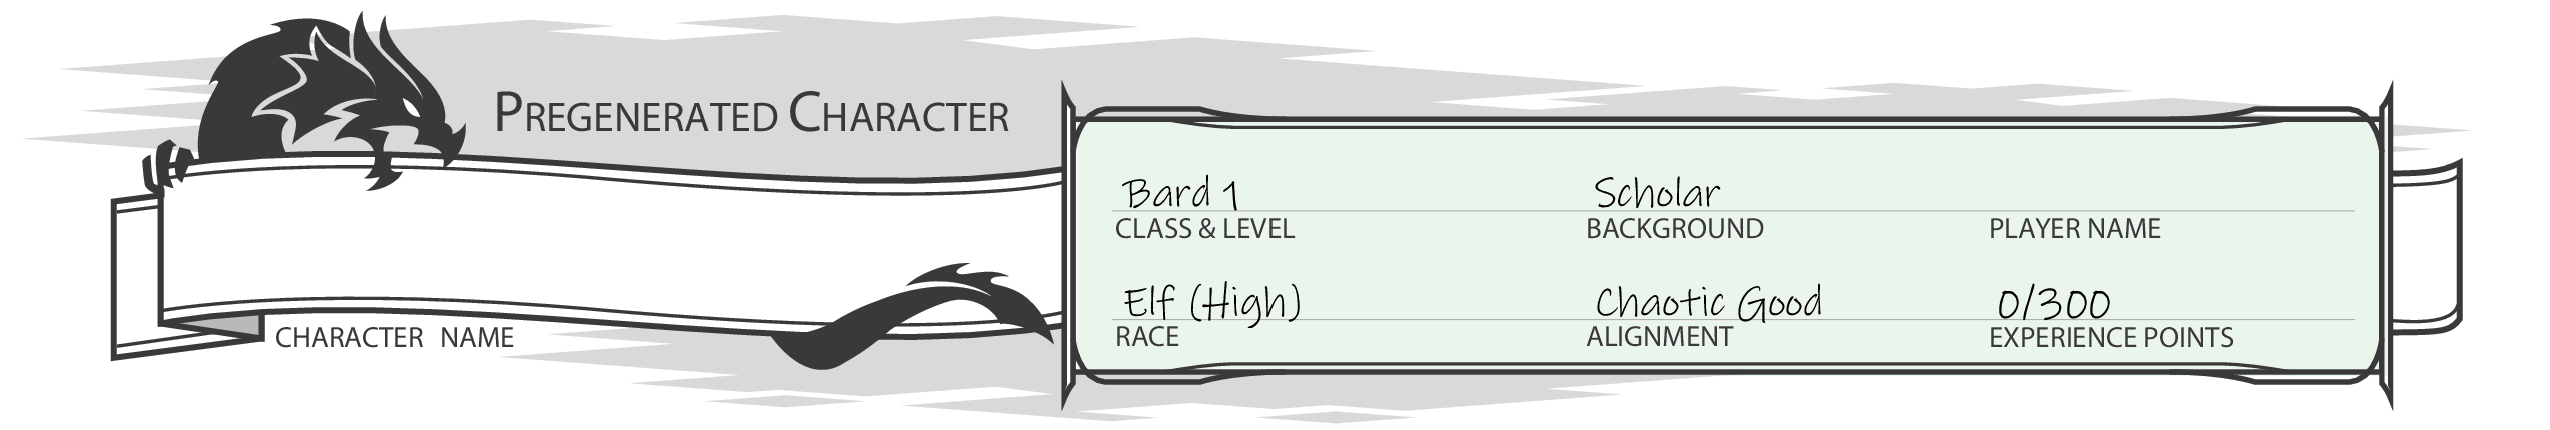
\includegraphics[width=\textwidth]{splash.png}};


  \begingroup\sffamily\Large

      \node (hpbackground) 
        [outer sep=0pt,fill=hpetc,below right corner=of splash,width=102mm, minimum height=46mm] 
       { };

      \node (hitdice)
             [dndhits,width=20mm,inside south east corner=of hpbackground,
             dndlabel=HIT DICE] 
         { \Large d8 }
         ;

      \node (curhp)
            [dndhits,fill=white,width=72mm,left=of hitdice,
             dnd/label={CURRENT HIT POINTS}] 
         { \Large \bfseries\sffamily 10 }
         ;

      \node [dndmaxhp,above left corner=of curhp,dndlabel=MAX HP] 
         (maxhp)
         { \Large 99 }
         ;

      \node (initiative)
            [dndmaxhp,right=of maxhp,dndlabel=INITIATIVE] 
         { +2 }
         ;

      \node (speed)
            [dndmaxhp,right=of initiative,dndlabel=SPEED] 
         { 30~ft }
         ;


       \node (ac) [dndmaxhp,shield,innershield,draw,ultra thick,right=of speed,width=15mm,
                   dndlabel={\noexpand\tinystacklabel{ARMOR}{CLASS}},
            ]
      {\raisebox{4mm}{13}}
      ;

  \endgroup


\begin{attacks}[below right corner=of hpbackground]{}
    \centering
    \begin{attackstab}
    Shortsword & +4 & 1d6+2 & piercing & 5 ft. & ---\\
    Hand Axe (off~hand) [B]& +5 & 1d6 & slashing & 5~ft or 20/60~ft& ---\\
    \end{attackstab}
\end{attacks}


% \node (attacks) at (hpbackground.south west) {A};

\begin{magic}[below=of attacks]{}
\centering
\begin{featurestab}
% Magic section (right side, middle)
  \textsf{CANTRIPS}\\
  Friends& Does a thing\\
  Ray of Frost& asdf\\
  \multicolumn2{l}{\textsf{1st-LEVEL SPELLS \spellslots{3}}}\\
\end{featurestab}
\end{magic}


\begin{features}[below=of magic]{}
\begin{featurestab}
\feature{Fey Ancestry}{
  You have advantage to save against charms and you can't be magically put to sleep.}
\feature{\centering Bardic~Inspiration (2/day)}
 {Grant an ally within 60 ft +1d6 inspiration they can use on any one check within 10 minutes.}
\feature{Ritual Caster}{    
  Cast certain spells as 10-minute rituals instead of using a spell slot.}
\end{featurestab}
\end{features}

\node (stats background) 
      [fill=stats,width=24mm,height=163mm,below left corner=of splash] { };

\stat{STRENGTH}{10}
\stat*{DEXTERITY}{15}
\stat{CONSTITUTION}{8}
\stat{INTELLIGENCE}{15}
\stat{WISDOM}{12}
\stat*{CHARISMA}{15}

  
\begin{equipment}[below left corner=of stats background]
    \item Clothes (Fine)
    \item Leather Armor
    \item Shortsword
    \item Lyre
    \item Backpack
    \item Bedroll, Book of Elvish Poetry
    \item Bottle of Ink, Ink Pen
    \item Parchment (10 sheets), Tinderbox
    \item Trail Rations (10 days), Waterskin
\end{equipment}

\path (equipment.north west) +(3mm,-4mm) coordinate (coin top left);

\tikzset{coin/.style={
   dndbox,
   long octagon,
   long octagon angle=45,
   long octagon end height=2.5mm,
   width=15.5mm,
   height=7.5mm
}}

\node (cp) [coin,anchor=north west,at=(coin top left)] {10};
\node (sp) [coin,below=of cp] {5};
\node (ep) [coin,below=of sp] {};
\node (gp) [coin,below=of ep] {10};
\node (pp) [coin,below=of gp] {};


%\begin{equipmentx}[right=of equipment]
%    \item Clothes (Fine)
%    \item Leather Armor
%    \item Shortsword
%    \item Lyre
%    \item Backpack
%    \item Bedroll, Book of Elvish Poetry
%    \item Bottle of Ink, Ink Pen
%    \item Parchment (10 sheets), Tinderbox
%    \item Trail Rations (10 days), Waterskin
%\end{equipmentx}

  
\node (proficiency bonus)
      [proficiencies,decorated stub rectangle,width=38mm,height=8mm,
       right of upper corner=3.5mm of stats background]
   {\hbox to 0pt{\hss\hspace*{9mm}\tiny\textsf{PROFICIENCY BONUS}\hss}}
   ;
\node [anchor=west,proficiencies,circle,
       width=10mm,height=10mm,line width=1.5pt,draw]
       at ($(proficiency bonus.west)+(-2mm,0mm)$)
      {\large\textsf{+\arabic{proficiency bonus}}};

% Proficiencies section (middle top)
\begin{proficiencies}[below=of proficiency bonus,width=38mm]
  \small
\item
  {Acrobatics}
\item
  Arcana
\item
  History
\item
  Investigation
\item
  Perception
\item
  Performance
\item
  Persuasion
\item
  Musical Instrument (Lyre)
\item
  Language (Common)
\item
  Language (Elvish)
\end{proficiencies}

\node (passive perception)
   [dndmaxhp,left=10mm of maxhp,width=24mm] 
   {\Large\textsf{13}}
   ;

\dndlabel{passive perception}{\pplabel}

\node (senses)
   [dndmaxhp,left=10mm of curhp,width=24mm] 
   {\itshape\begin{tabular}{c}{Darkvision}\\{60~ft}\\[3pt]\end{tabular}}
   ;
\dndlabel{senses}{\scriptsize SENSES}


\end{charsheet}




\end{document}
